%% The following is a directive for TeXShop to indicate the main file
%%!TEX root = diss.tex

% TODO: Make sure I pick a value that matches up (y-axis)

\subfloat[]{%
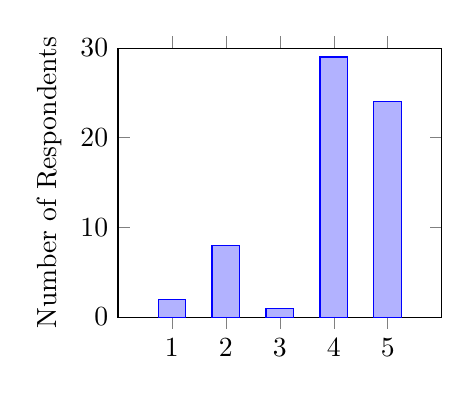
\begin{tikzpicture}
\begin{axis}[
    ybar=0pt,
    scale = 0.6,
    /pgf/number format/1000 sep={},
    xticklabels={1, 2, 3, 4, 5},
    xtick = {1,2,3,4,5},
    ymin = 0,
    ymax = 30,
    ylabel = {Number of Respondents},
    enlarge x limits=0.25
]
\addplot coordinates {
    (1, 2) (2, 8) (3, 1) (4, 29) (5, 24)
};
\end{axis}
\end{tikzpicture}%
}

\subfloat[]{%
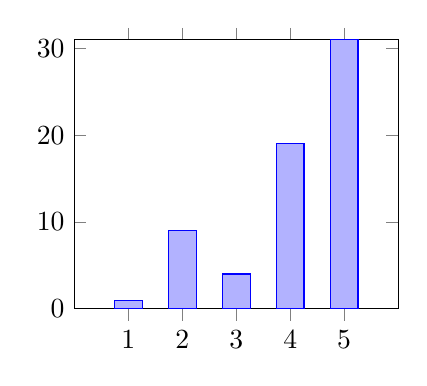
\begin{tikzpicture}
\begin{axis}[
    ybar=0pt,
    scale = 0.6,
    /pgf/number format/1000 sep={},
    xticklabels={1, 2, 3, 4, 5},
    xtick = {1,2,3,4,5},
    ymin = 0,
    ymax = 31,
    enlarge x limits=0.25
]
\addplot coordinates {
    (1, 1) (2, 9) (3, 4) (4, 19) (5, 31)
};
\end{axis}
\end{tikzpicture}%
}

\subfloat[]{%
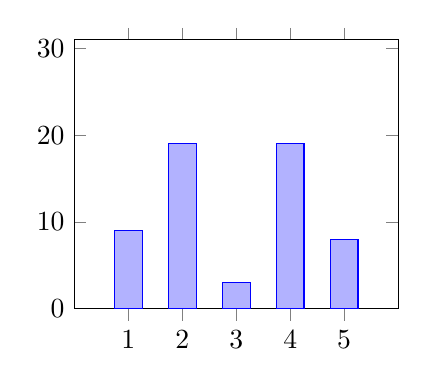
\begin{tikzpicture}
\begin{axis}[
    ybar=0pt,
    scale = 0.6,
    /pgf/number format/1000 sep={},
    xticklabels={1, 2, 3, 4, 5},
    xtick = {1,2,3,4,5},
    ymin = 0,
    ymax = 31,
    enlarge x limits=0.25
]
\addplot coordinates {
    (1, 9) (2, 19) (3, 3) (4, 19) (5, 8)
};
\end{axis}
\end{tikzpicture}%
}

% TODO: this blows up
% \subfloat[]{%
% \begin{tikzpicture}
% \begin{axis}[
%     ybar=0pt,
%     scale = 0.6,
%     /pgf/number format/1000 sep={},
%     xticklabels={1, 2, 3, 4, 5},
%     xtick = {1,2,3,4,5},
%     ymin = 0,
%     ymax = 31,
%     enlarge x limits=0.25
% ]
% \addplot coordinates {
%     (1, 4) (2, 15) (3, 3) (4, 23) (5, 8)
% };
% \end{axis}
% \end{tikzpicture}%
% }

